\documentclass{jfp}

%%%%%%%%%%%%%%%%%%%%%%%%%%%%%%%%%%%%%%%%%%%%%%%%%%%%%%%%%%%%
% Global switches
%%%%%%%%%%%%%%%%%%%%%%%%%%%%%%%%%%%%%%%%%%%%%%%%%%%%%%%%%%%%

% Turn on to include todos and comments.  These are intended for stuff
% we need to do or discussions that may influence the text of the
% paper itself.
\newif\ifcomments\commentstrue

% Turn on to include commentary. This is intended for stuff we want to
% remember/write down but do not intend to include in the paper.
\newif\ifcommentary\commentarytrue

%%%%%%%%%%%%%%%%%%%%%%%%%%%%%%%%%%%%%%%%%%%%%%%%%%%%%%%%%%%%
% Packages
%%%%%%%%%%%%%%%%%%%%%%%%%%%%%%%%%%%%%%%%%%%%%%%%%%%%%%%%%%%%

\usepackage[T1]{fontenc}
\usepackage[utf8]{inputenc}
\usepackage[override]{cmtt}
\usepackage{hyperref}
\usepackage{mdframed}
\usepackage{comment}
\usepackage[svgnames]{xcolor}

\usepackage{graphicx}
\graphicspath{{images/}}

\usepackage{latex/agda}
% for grabbing pieces of Agda from a different file, so that latex and
% Agda don't have to mix too much.
\usepackage{catchfilebetweentags}

% Typeset Agda comments in normal roman text, offset by a qquad of
% space, instead of using texttt
\renewcommand{\AgdaCommentFontStyle}[1]{\qquad #1}

\usepackage[backend=pgf, outputdir=diagrams]{diagrams-latex}
\usepackage{pgf}

%%%%%%%%%%%%%%%%%%%%%%%%%%%%%%%%%%%%%%%%%%%%%%%%%%%%%%%%%%%%
% Unicode
%%%%%%%%%%%%%%%%%%%%%%%%%%%%%%%%%%%%%%%%%%%%%%%%%%%%%%%%%%%%

% See https://agda.readthedocs.io/en/v2.6.0.1/tools/generating-latex.html

\usepackage{newunicodechar}
\newunicodechar{∀}{\ensuremath{\forall}}
\newunicodechar{ℓ}{\ensuremath{\ell}}
\newunicodechar{→}{\ensuremath{\to}}
\newunicodechar{λ}{\ensuremath{\lambda}}
\newunicodechar{ℕ}{\ensuremath{\mathbb{N}}}
\newunicodechar{∘}{\ensuremath{\circ}}
\newunicodechar{′}{\ensuremath{{}^\prime}}
\newunicodechar{⊔}{\ensuremath{\sqcup}}

%%%%%%%%%%%%%%%%%%%%%%%%%%%%%%%%%%%%%%%%%%%%%%%%%%%%%%%%%%%%
% Typesetting
%%%%%%%%%%%%%%%%%%%%%%%%%%%%%%%%%%%%%%%%%%%%%%%%%%%%%%%%%%%%

\newcommand{\term}[1]{\emph{#1}}

%%%%%%%%%%%%%%%%%%%%%%%%%%%%%%%%%%%%%%%%%%%%%%%%%%%%%%%%%%%%
%% Comments
%%%%%%%%%%%%%%%%%%%%%%%%%%%%%%%%%%%%%%%%%%%%%%%%%%%%%%%%%%%%

\ifcomments
\newcommand{\authornote}[3]{\textcolor{#1}{[#3 ---#2]}}
\newcommand{\todo}[1]{\textcolor{red}{[TODO: #1]}}
\else
\newcommand{\authornote}[3]{}
\newcommand{\todo}[1]{}
\fi

\newcommand{\bay}[1]{\authornote{blue}{BAY}{#1}}
\newcommand{\jc}[1]{\authornote{green}{JC}{#1}}  % pick whatever
                                                 % color/initials you want

\ifcommentary
  \newmdenv[skipabove=1em, skipbelow=1em, innermargin=1.5em, outermargin=1.5em, backgroundcolor=black!8, linecolor=black!10]{commentary}
\else
  \excludecomment{commentary}
\fi

%%%%%%%%%%%%%%%%%%%%%%%%%%%%%%%%%%%%%%%%%%%%%%%%%%%%%%%%%%%%
% Front matter
%%%%%%%%%%%%%%%%%%%%%%%%%%%%%%%%%%%%%%%%%%%%%%%%%%%%%%%%%%%%

\title{Memory Models via Species: The Paper}
\subtitle{Or: You Could Have Invented Species, If You Happened To Think
  About It In This Very Specific Way}
\author[J. Carette and B. A. Yorgey]{JACQUES CARETTE\\
  McMaster University, Ontario, Canada \\
  \email{carette@mcmaster.ca}
  \and BRENT A. YORGEY\\
  Hendrix College, Arkansas, USA\\
  \email{yorgey@hendrix.edu}}

%%%%%%%%%%%%%%%%%%%%%%%%%%%%%%%%%%%%%%%%%%%%%%%%%%%%%%%%%%%%

\begin{document}

\maketitle

\jc{I don't think we should put Species, the word,
  in the title at all. I have no problems with using the current
  title as the working title, but we'll see how things develop.}
\bay{Agreed!}

What is a \term{memory}?  For our purposes, a memory is \emph{a store
  of values}, that is, an abstract container where values can be
stored and later retrieved.

\begin{commentary}
  This used to say ``a collection of locations where
values can be stored and later retrieved'', but that is, in some
ways, double indirection -- at least it will be as soon as labels
are introduced.  I'm not so sure about the word ``container'', but
that can be figured out later.
\end{commentary}

What sort of structure does a memory need to have to make this
possible?  If there are to be many values stored in a memory, and we
want to somehow retrieve a particular value, how can we do that?
There must be some way to refer to individual values in the memory, so
we suppose that we have some collection of \emph{labels} which can be
used for that purpose. Then a memory is just a way to associate
values to labels.

\begin{figure}[htp]
  \centering
  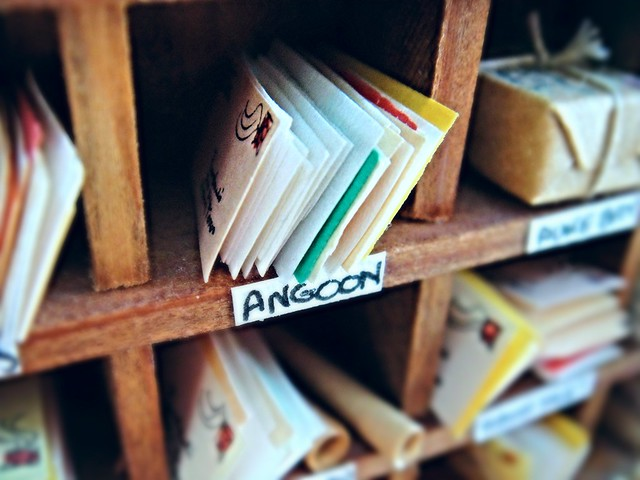
\includegraphics[width=0.5\textwidth]{mailboxes.jpg}
  \caption{A memory with labelled values. Photo by JLS Photography.\protect\footnotemark}
  \label{fig:mailboxes}
\end{figure}
\footnotetext{\url{https://www.flickr.com/photos/akgypsy37/8690531067/}, CC BY-NC-ND 2.0.}

\begin{commentary}
  The intent of the picture is to show a very physical
notion of ``labelled memory'', where the labels are quite
visible, and there are physical things ``stored'' at the address
indicated by the label.
\end{commentary}

One simple model of a memory is therefore a \emph{function} from the
set of possible labels to the set of possible values. To retrieve a
value with a particular label is to simply evaluate the function at a
particular input label.  However, this is certainly not the only
possible model.

\begin{commentary}
  There is a subtle issue with the next paragraph: in the picture it
  is actually the \emph{locations} which are in a 2D grid; the
  \emph{labels} themselves (presumably) do not reflect this structure.
  Ultimately, the concept of ``locations'' is there as a conceptual
  aid, but is not directly reflected in our framework.  In the
  physical world, one could take the physical coordinates of locations
  (relative to some reference) as a set of labels, and then going from
  (what we would usually think of as) a ``label'' to physical
  coordinates is accomplished by a final relabelling operation, where
  the ``relabelling'' isomorphism is actually (in one direction) an
  algorithm for doing some sort of physical search.  For example, if
  you know the call number (one set of labels) of a book in a library,
  the facts that (1) the call numbers have a total ordering and (2)
  the books are arranged in physical space in a particular way
  according to the ordering---i.e. there is an \emph{order-preserving
    isomorphism} between call numbers and physical locations---means
  that you can perform something like a binary search in physical
  space to find the physical location (another set of labels) of the
  book you want.  (To compute the other direction of the isomorphism,
  of course, you just look at the call number printed on the spine of
  a book---though it's interesting/notable that in the case of a
  library it's actually the \emph{values} (i.e. books) that are
  labelled with call numbers rather than the locations themselves.
  Declining to label the locations with call numbers is an
  optimization that allows for easier compaction/garbage
  collection\dots) It's interesting that to carry out one direction of
  the isomorphism (call number -> physical location) requires
  repeatedly running it in the opposite direction (pick a physical
  location, find the call number of the book there, and compare to
  your chosen call number to decide which direction to go next).

  In RAM, of course, the last relabelling to convert a physical
  address into a physical location doesn't use search, but rather a
  circuit which selects a physical location based on the bit pattern
  used to encode the address.  This relabelling is also
  order-preserving in a certain sense, though that's only because it
  leads to a nice/efficient/concise circuit; there's no a priori
  reason we couldn't build a circuit which maps consecutive addresses
  to arbitrary non-consecutive physical locations.
\end{commentary}

For now, we don't assume that labels have any special structure
(though some particular sets of labels might).  For example, the
labels in Figure~\ref{fig:mailboxes} are evidently arranged in a 2D
grid, but this is a special case.  In the abstract, it may be helpful
to imagine a memory as a ``soup'' of labelled values, where the labels
are completely arbitrary.  As an illustration, Figure~\ref{fig:soup}
shows a memory with three labelled values. The values are not
arranged in any particular relation to one another; moreover, the
labels have been chosen to emphasize that the set of labels can be
entirely arbitrary, without any sort of inherent structure.  The
labels may or may not have decidable equality, may or may not be
concretely representable as sequences of bits, and so on.

\begin{figure}
  \centering
  \begin{diagram}[width=150]
  drawLocation :: Diagram B -> Diagram B -> Diagram B
  drawLocation lab val = vsep 0.2 [val <> roundedRect 1 1 0.1, lab]

  locs cow = zipWith drawLocation
    [ circle 0.2 # fc blue # lw none
    , text "$\\alpha$" # fontSizeL 0.5 <> phantom (square 0.5 :: D V2 Double)
    , image cow # sized (dims (1 ^& 1))
    ]
    (map (fontSizeL 0.8 . text . show) [2, 7, 5])

  cs =
    [ origin
    , 3 ^& (-2)
    , 4 ^& 1
    ]

  dia :: IO (Diagram B)
  dia = do
    Right cow <- loadImageEmb ("images/cow.png")
    return $ mconcat (zipWith moveTo cs (locs cow))  -- $
  \end{diagram}
  \caption{A ``soup'' of labelled integer values}
  \label{fig:soup}
\end{figure}

We will use Agda \todo{cite} as a concrete metalogic in which to
express our ideas.  For example, we can encode the simple function
model of memory, discussed above, as follows:

\ExecuteMetaData[latex/models.tex]{naivememory}

Throughout the rest of the paper, we will use Agda's
\AgdaKeyword{variable} feature to declare that certain common
variables should be implicitly generalized whenever they occur free in
a type.  This way, we can avoid tediously specifying them as implicit
parameters at the beginning of every single type signature.
\ExecuteMetaData[latex/models.tex]{variable}
%
For example, using these implicitly generalized variables, we can
rewrite \AgdaFunction{MemoryF} and \AgdaFunction{lookupF} as
follows:
%
\ExecuteMetaData[latex/models.tex]{naivememory2}

It is important to bear in mind that although we use Agda as a way to
conveniently express our ideas, we make no particular commitments to
the specific metalogic used and what features it may or may not have
available.  For example, Agda has many built-in type formers (sums,
products, \emph{etc.}) which allow one to construct new types out of
existing ones, but we will not take such type formers for granted.  In
general, the name of the game is to add structure in a gradual,
carefully controlled manner, so as to discover the minimum amount of
structure necessary to model various phenomena.

\begin{commentary}
  In fact what we are committing to up front is simply a category
  where objects are types, with some notion of morphisms between
  types, but we will get to this much later.
\end{commentary}

By the same token, we don't want to commit up front to any particular
model of a memory.  Instead of defining \AgdaFunction{Memory} as one
particular model or another, we can define it as an Agda record which
specifies the abstract interface that any model of memory should
provide.  So far, we require only two things of a model: a type
\AgdaField{Mem} representing the model itself, and a function
\AgdaField{lookup} allowing us to retrieve the value associated to a
particular label.  We will add more fields to this record as we
discover more structure we wish to impose on our notion of memory.
%
\ExecuteMetaData[latex/models.tex]{memrecord}
%
For example, we can verify that functions are a valid model of memory
so far:
%
\ExecuteMetaData[latex/models.tex]{fnasmemory}

\subsection{Relabelling}
\label{sec:relabelling}

The next operation we require is \emph{relabelling}: it should be
possible to exchange the set of labels for a new set.  Conceptually,
the reason to require such an operation is that the specific labels
used ``shouldn't matter'': the labels are only there to give us a way
to retrieve specific values.  Thus, two memories with the same values
but different labels should in some sense be interchangeable (though
of course they are not identical).

Talk of ``exchanging'' label sets might suggest that we should be
required to relabel with a new label set \emph{of the same size} as
the old, with a specified one-to-one mapping between them.  And
indeed, in some situations we might want to restrict relabelling in
exactly this way.  However, a more general version of relabelling
allows us to model some interesting phenomena; we will return to
discuss the distinction in more detail later.  For now, we introduce a
new \AgdaField{relabel} operation as follows:
\ExecuteMetaData[latex/models.tex]{memrecord-relabel} Note that the
relabelling function is ``backwards'' (\emph{i.e.} contravariant),
that is, it maps new labels to old.  This may be surprising on one
level, since when we think about replacing one set of labels by
another we intuitively imagine a mapping \emph{from} the old set of
labels \emph{to} the new ones. However, it becomes clear that
contravariance is required if we want to retain the simple model of
memory as a function:

\ExecuteMetaData[latex/models.tex]{fnasmemory-relabel}

If memory is a function mapping labels to values, then in order to
relabel we need a way to translate new labels to old, which we
precompose with the memory mapping itself.  When given a new label to
look up, we first run it through the given function to translate it
into a corresponding old label, then look up the old label in the
underlying memory.

\begin{commentary}
  This used to say that relabelling essentially amounts to saying that
  Mem is a contravariant functor in the label argument, but as Jacques
  correctly points out it is not quite there yet: there are some extra
  properties we would need too.

  ``\dots after relabelling, all you need is to consider functions on
  $V$ as being interesting (and in programming, you often want to
  apply functions to values, regardless of 'memory'). That is enough
  to pack everything together into Categories + Functors.''
\end{commentary}

Looking at the picture in Figure~\ref{fig:mailboxes}, we might intuitively
visualize relabelling in terms of phyiscally replacing the old labels
with new ones. However, the foregoing discussion suggests there is
another way to think of it: instead of \emph{replacing} the labels we
can simply store a function off to the side.  In terms of the picture,
we might imagine having a little book sitting next to the mailboxes in
which you can look up a name and see which actual name it corresponds
to on the mailboxes.

\todo{picture of relabelling}

In fact, there are real-world memory systems that work this way.  For
example, virtual memory works by maintaining a mapping from virtual
addresses to physical addresses (a \term{page table}); when a process
requests the value at a particular address, the address is first
translated to a physical address using the mapping, and then
the resulting physical address is looked up in memory.
\begin{commentary}
  Paging memory to and from disk complicates this story somewhat.  I
  have not thought about it too carefully yet but I think it
  corresponds to applying a relabelling operation to the physical
  memory directly.  That is, suppose we have a physical memory
  $M : Mem\; PA\; Bits$ (comprising both RAM and disk), where $PA$ is
  the type of physical addresses.  Then a virtual memory system
  results from applying a relabelling of type $VA \to PA$ that
  translates virtual addresses to physical addresses.  But to
  represent/implement swapping you have to intensionally know that
  this virtual memory system is represented as a pair $(PT, M)$ where
  $PT : VA \to PA$ is the page table.  Then swapping corresponds to
  applying a permutation relabelling $\varphi : PA \to PA$ directly to
  $M$, resulting in the new virtual memory
  $(PT, \mathit{relabel}\; \varphi\; M)$.  Of course, application of
  $\varphi$ is implemented by physically copying stuff around rather
  than storing a function off to the side.
\end{commentary}
Another example is \todo{array libraries}

\begin{itemize}
\item The relabelling function might not be surjective, that is, some
  of the old labels might be left out. This allows us to model
  deleting or ``freeing'' memory that is no longer needed.
\item Likewise, the relabelling function might not be injective, that
  is, multiple new labels may map to the same old label.  This allows
  us to model aliasing.

  ``bags for free''.

  ``aliasing'' is a loaded term!  Implies mutability, i.e. assign
  operation.  Leave that until later.
\end{itemize}

\begin{commentary}
  relabel is still useful if $L' = L$.  e.g. Copying garbage collection.
\end{commentary}

\begin{commentary}
Note that a $\AgdaFunction{Memory}$ must be a \emph{total} function,
that is, every label corresponds to some value.  If we wish to model
memories where some labels do not correspond to a stored value, we can
simply use a type $V$ of values with a distinguished ``empty'' value.
\todo{Actually there are other choices too!  e.g. get rid of labels
  entirely.  This is why we're going to wait.}
\end{commentary}

\todo{eventual motivation: represent data structures!  So we need some
  structure on labels (?)  Next up: disjoint union.  Related to
  malloc: what to do if someone hands you some new labels.  Look at
  haskell/src/Data/Storage.hs If you have two memories and want to put
  them together, you definitely need disjoint union of label sets:
  otherwise when handed a label there's no way to know which memory to
  do lookup on.  Is there a compatibility law with disjoint union and
  relabel?  Note we can always put two relabelling maps together into
  one on a disjoint union, but can we go in the other direction?
  Requires bijections?}

\begin{commentary}
  Models with and without functoriality for values!  Might have to do
  something like co-Yoneda trick to make it functorial.
\end{commentary}

\bay{At some point in the future we will want to talk about label
  equality, but not yet.  Don't you need decidable equality at the
  point where you want a ``set'' operation (i.e. an operation that
  takes a memory, a label, and a (new) value, and sets the value at
  the given location, returning a new updated memory)?}

\subsection{Label equality}
\label{sec:label-equality}

As an example, take $L = \mathbb{R}$ to be the set of real numbers.
A ``memory'' with this set of labels is thus an assignment of a value
to every point on the real line.

Although this is well-defined, it is hard to imagine how one could
actually do anything with such a memory.  The problem is that
\bay{how to say exactly what the problem is?  Is this actually a good
  example?  It seems like it may actually be combining several
  problems (uncountable number of elements; uncomputable elements; no
  decidable equality\dots)}

We will thus usually want to limit ourselves to label sets $L$ which
come with a decidable equivalence relation, and require that the
mapping from labels to values respects this equivalence (that is,
equivalent labels are never mapped to different values).

\bay{What Agda code should go along with this?}


\begin{commentary}
  Simplest data structure: singleton-indexed.  Next: two-element-set
  indexed, i.e. a pair.  Note it is not necessarily an ORDERED pair!
  Talk about relabelling, functoriality, groupoids...

  Distinction between single structures and *collections* of
  structures (aka species aka data types).

  'assign' operation requires decidable equality?

  Laws for lookup/assign?  Interacts with what kind of relabelling is
  allowed.
\end{commentary}

\end{document}
